%% LyX 1.6.7 created this file.  For more info, see http://www.lyx.org/.
%% Do not edit unless you really know what you are doing.
\documentclass[english]{beamer}
\usepackage{mathptmx}
\usepackage[T1]{fontenc}
\usepackage[latin9]{inputenc}
\usepackage{color}
\usepackage{babel}

\usepackage{url}
\usepackage{amsmath}
\usepackage{graphicx}
\usepackage{amssymb}
\hypersetup{unicode=true, pdfusetitle,
 bookmarks=true,bookmarksnumbered=false,bookmarksopen=false,
 breaklinks=false,pdfborder={0 0 1},backref=false,colorlinks=false,}

\makeatletter

%%%%%%%%%%%%%%%%%%%%%%%%%%%%%% LyX specific LaTeX commands.
\newcommand{\noun}[1]{\textsc{#1}}
%% Because html converters don't know tabularnewline
\providecommand{\tabularnewline}{\\}

%%%%%%%%%%%%%%%%%%%%%%%%%%%%%% Textclass specific LaTeX commands.
 % this default might be overridden by plain title style
 \newcommand\makebeamertitle{\frame{\maketitle}}%
 \AtBeginDocument{
   \let\origtableofcontents=\tableofcontents
   \def\tableofcontents{\@ifnextchar[{\origtableofcontents}{\gobbletableofcontents}}
   \def\gobbletableofcontents#1{\origtableofcontents}
 }
 \makeatletter
 \long\def\lyxframe#1{\@lyxframe#1\@lyxframestop}%
 \def\@lyxframe{\@ifnextchar<{\@@lyxframe}{\@@lyxframe<*>}}%
 \def\@@lyxframe<#1>{\@ifnextchar[{\@@@lyxframe<#1>}{\@@@lyxframe<#1>[]}}
 \def\@@@lyxframe<#1>[{\@ifnextchar<{\@@@@@lyxframe<#1>[}{\@@@@lyxframe<#1>[<*>][}}
 \def\@@@@@lyxframe<#1>[#2]{\@ifnextchar[{\@@@@lyxframe<#1>[#2]}{\@@@@lyxframe<#1>[#2][]}}
 \long\def\@@@@lyxframe<#1>[#2][#3]#4\@lyxframestop#5\lyxframeend{%
   \frame<#1>[#2][#3]{\frametitle{#4}#5}}
 \makeatother
 \def\lyxframeend{} % In case there is a superfluous frame end

%%%%%%%%%%%%%%%%%%%%%%%%%%%%%% User specified LaTeX commands.
\usetheme{Warsaw}
% or ...

\setbeamercovered{transparent}
% or whatever (possibly just delete it)

\makeatother

\begin{document}

\title{Data Serialization}


\subtitle{From pickle to databases and HDF5}


\author{Francesc~Alted}


\institute{Freelance Developer and PyTables Creator}


\date[2010 Autumn School

]{Advanced Scientific Programming in Python\\
2010 Autumn School, Trento, Italy }

\makebeamertitle


%\pgfdeclareimage[height=3.5cm]{logo}{logo.pdf}

%\logo{\pgfuseimage{logo}}



\AtBeginSubsection[]{

  \frame<beamer>{ 

    \frametitle{Outline}   

\tableofcontents[currentsection,currentsubsection] 
%\tableofcontents[currentsubsection] 

  }

}



%\beamerdefaultoverlayspecification{<+->}


\lyxframeend{}\lyxframe{Outline}

\tableofcontents{}


\lyxframeend{}\section{The Basics}


\lyxframeend{}\subsection{Introduction}


\lyxframeend{}\lyxframe{What {}``serialization'' means?}
\begin{quotation}%{}
{}``Serialization is the process of converting a data structure or
object into a sequence of bits so that it can be stored in a file
or memory buffer, or transmitted across a network connection link
to be \textquotedbl{}resurrected\textquotedbl{} later in the same
or another computer environment.''

{}``The basic mechanisms are to flatten object(s) into a one-dimensional
stream of bits, and to turn that stream of bits back into the original
object(s).''\end{quotation}%{}
\begin{verse}%{}
-- From http://www.parashift.com/c++-faq-lite/serialization.html
\end{verse}%{}

\lyxframeend{}\lyxframe{Serialization tools}

There are literally zillions of serialization tools and formats (text,
XML, or binary based), but well be focusing on those that are:
\begin{itemize}
\item Easy to use
\item Space-efficient
\item Fast
\end{itemize}
In particular, we are not going to discuss text-based formats (e.g.
XML, CSV, JSON, YAML ...).


\lyxframeend{}\lyxframe{Serialization tools that comes with Python}

Python comes with a complete toolset of modules for serialization
purposes:
\begin{itemize}
\item pickle, and its cousin, cPickle, for quick-and-dirty serialization.
\item shelve, a persistent dictionary based on DBM databases.
\item A common database API for communicating with relational databases.
\end{itemize}

\lyxframeend{}\lyxframe{Serialization tools for binary data}

Additionally, there are lots of third-party libraries for specialized
uses. Here will center on numerical formats:
\begin{itemize}
\item NPY, NPZ: NumPy own's format.
\item Wrappers for HDF5, a standard de-facto format and library: PyTables,
h5py.
\item Wrappers for NetCDF4, a widely used library based on HDF5: netcdf4-python,
Scientific.IO.NetCDF.
\end{itemize}

\lyxframeend{}\subsection{Pickling our objects}


\lyxframeend{}\lyxframe{The \texttt{pickle} module}

Serializes an object into a stream of bytes that can be saved to a
file and later restored:
\begin{example}%{}


\texttt{\footnotesize import pickle}{\footnotesize \par}

\texttt{\footnotesize obj = SomeObject()}{\footnotesize \par}

\texttt{\footnotesize f = open(filename, 'wb')}{\footnotesize \par}

\texttt{\footnotesize pickle.dump(obj, f)}{\footnotesize \par}

\texttt{\footnotesize f.close()}{\footnotesize \par}

\texttt{\footnotesize \# ... later on}{\footnotesize \par}

\texttt{\footnotesize import pickle}{\footnotesize \par}

\texttt{\footnotesize f = open(filename, 'rb')}{\footnotesize \par}

\texttt{\footnotesize obj = pickle.load(f)}{\footnotesize \par}

\texttt{\footnotesize f.close()}{\footnotesize \par}


\end{example}%{}

\lyxframeend{}\lyxframe{What \texttt{pickle} does}
\begin{itemize}
\item It can serialize both basic Python data structures or user-defined
classes.
\item Always serializes data, not code (it tries to import classes if found
in the pickle).\end{itemize}
\begin{alertblock}
{}For security reasons, programs should not unpickle data received
from untrusted sources.
\end{alertblock}

\lyxframeend{}\lyxframe{Its \texttt{cPickle} cousin}
\begin{itemize}
\item Implemented in C (i.e. significantly faster than \texttt{pickle}).
\item But more restrictive (does not allow subclassing of the \texttt{Pickler}
and \texttt{Unpickler} objects).
\item Python 3 \texttt{pickle} can use the C implementation transparently.
\end{itemize}

\lyxframeend{}\lyxframe{Pickling a NumPy array}

\texttt{\footnotesize >\textcompwordmark{}>\textcompwordmark{}> a
= np.linspace(0, 100, 1e7)}{\footnotesize \par}

\texttt{\footnotesize ~}{\footnotesize \par}

\texttt{\footnotesize >\textcompwordmark{}>\textcompwordmark{}> time
pickle.dump(a, open('p1','w'))}{\footnotesize \par}

\texttt{\footnotesize CPU times: user 5.89 s, sys: 0.59 s, total: 6.48
s}{\footnotesize \par}

\texttt{\footnotesize ~}{\footnotesize \par}

\texttt{\footnotesize >\textcompwordmark{}>\textcompwordmark{}> time
pickle.dump(a, open('p2','w'), pickle.HIGHEST\_PROTOCOL)}{\footnotesize \par}

\texttt{\footnotesize CPU times: user 0.05 s, sys: 0.12 s, total: 0.16
s}{\footnotesize \par}

\texttt{\footnotesize ~}{\footnotesize \par}

\texttt{\footnotesize >\textcompwordmark{}>\textcompwordmark{}> time
cPickle.dump(a, open('p3','w'), pickle.HIGHEST\_PROTOCOL)}{\footnotesize \par}

\texttt{\footnotesize CPU times: user 0.02 s, sys: 0.08 s, total: 0.11
s}{\footnotesize \par}

\texttt{\footnotesize ~}{\footnotesize \par}

\texttt{\footnotesize >\textcompwordmark{}>\textcompwordmark{}> ls
-sh p1 p2 p3}{\footnotesize \par}

\texttt{\footnotesize 186M p1 77M p2 77M p3 }{\footnotesize \par}

~
\begin{block}
{}Always try to use \texttt{cPickle} and \texttt{HIGHEST\_PROTOCOL}
\end{block}

\lyxframeend{}\lyxframe{\texttt{pickle/cPickle} limitations}
\begin{itemize}
\item You need to reload all the data in the pickle before you can use any
part of it. That might be inconvenient for large datasets.
\item Data can only be retrieved by other Python interpreters. You loose
data portability with other languages.
\item Not every object in Python can be serialized by \texttt{pickle} (e.g.
extensions).
\end{itemize}

\lyxframeend{}\lyxframe{Recommendations for using \texttt{pickle}}
\begin{itemize}
\item Use it mainly for small data structures.
\item If you have a lot of variables that you want to save, use a dictionary
for tying them together first.
\item When using the IPython shell, be sure to use the very convenient \texttt{\%store}
magic (it uses \texttt{pickle} under the hood).
\end{itemize}

\lyxframeend{}\lyxframe{The \texttt{shelve} module}
\begin{itemize}
\item Provides support for persitent objects using a special {}``shelf''
object.
\item The {}``shelf'' behaves like a disk-based dictionary (DBM-style).
\item The values of the dictionary can be any object that can be pickled.
\end{itemize}

\lyxframeend{}\lyxframe{Example with\texttt{ shelve}}

\texttt{\footnotesize >\textcompwordmark{}>\textcompwordmark{}> import
shelve}{\footnotesize \par}

\texttt{\footnotesize >\textcompwordmark{}>\textcompwordmark{}> }{\footnotesize \par}

\texttt{\footnotesize >\textcompwordmark{}>\textcompwordmark{}> db
= shelve.open(\textquotedbl{}database\textquotedbl{}, \textquotedbl{}c\textquotedbl{})}{\footnotesize \par}

\texttt{\footnotesize >\textcompwordmark{}>\textcompwordmark{}> db{[}\textquotedbl{}one\textquotedbl{}{]}
= 1}{\footnotesize \par}

\texttt{\footnotesize >\textcompwordmark{}>\textcompwordmark{}> db{[}\textquotedbl{}two\textquotedbl{}{]}
= 2}{\footnotesize \par}

\texttt{\footnotesize >\textcompwordmark{}>\textcompwordmark{}> db{[}\textquotedbl{}three\textquotedbl{}{]}
= 3}{\footnotesize \par}

\texttt{\footnotesize >\textcompwordmark{}>\textcompwordmark{}> db.close()}{\footnotesize \par}

\texttt{\footnotesize >\textcompwordmark{}>\textcompwordmark{}> }{\footnotesize \par}

\texttt{\footnotesize >\textcompwordmark{}>\textcompwordmark{}> db
= shelve.open(\textquotedbl{}database\textquotedbl{}, \textquotedbl{}r\textquotedbl{})}{\footnotesize \par}

\texttt{\footnotesize >\textcompwordmark{}>\textcompwordmark{}> for
key in db.keys():}{\footnotesize \par}

\texttt{\footnotesize ....: print repr(key), repr(db{[}key{]})}{\footnotesize \par}

\texttt{\footnotesize ....:}{\footnotesize \par}

\texttt{\footnotesize 'one' 1}{\footnotesize \par}

\texttt{\footnotesize 'two' 2}{\footnotesize \par}

\texttt{\footnotesize 'three' 3} 


\lyxframeend{}\lyxframe{Pros and cons of the \texttt{shelve} module}
\begin{block}
{Pros}Easy to retrieve just a selected set of variables.

Specially handy for large pickles.
\end{block}

\begin{block}
{Cons}Suffers the same problems than \texttt{pickle}\textrm{\emph{\noun{.}}}
\end{block}

\lyxframeend{}\subsection{Relational databases}


\lyxframeend{}\lyxframe{What's a relational database?}
\begin{itemize}
\item A set of tables containing data fitted into predefined categories.
\item Each table (a relation) contains one or more data categories in columns.
\item Each row contains a unique instance of data for the categories defined
by the columns.
\item Data can be accessed in many different ways without having to reorganize
the tables.
\end{itemize}

\lyxframeend{}\lyxframe{Terminology}

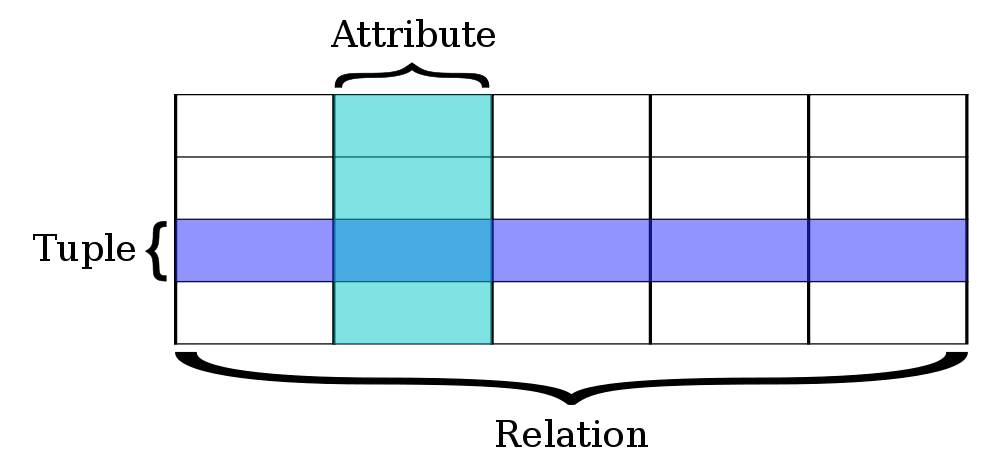
\includegraphics[scale=0.3]{Relational_database_terms}


\lyxframeend{}\lyxframe{Base and derived relations}
\begin{itemize}
\item In a relational database, all data are stored and accessed via relations.
\item Relations that store data are called \textquotedbl{}base relations\textquotedbl{},
and in implementations are called \textquotedbl{}tables\textquotedbl{}.
\item Other relations do not store data, but are computed by applying relational
operations to other relations.
\item These relations are sometimes called \textquotedbl{}derived relations\textquotedbl{}.
\item In implementations these are called \textquotedbl{}views\textquotedbl{}
or \textquotedbl{}queries\textquotedbl{}.
\end{itemize}

\lyxframeend{}\lyxframe{Example of relational database}

\begin{center}
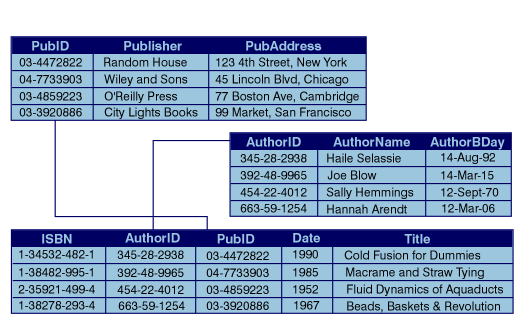
\includegraphics[scale=0.5]{example-reldatabase}
\par\end{center}


\lyxframeend{}\lyxframe{Queries with SQL language}

Simple query involving one single table (relation):
\begin{block}
{}

\texttt{\footnotesize SELECT AuthorName FROM AUTHORS WHERE AuthorBDay
> 1970}{\footnotesize \par}
\end{block}


Complex query involving multiple relations:
\begin{block}
{}

\texttt{\footnotesize SELECT AuthorName FROM AUTHORS a, BOOKS b, PUBLISHERS
p}{\footnotesize \par}

\texttt{\footnotesize ~~~~WHERE AuthorBDay > 1970}{\footnotesize \par}

\texttt{\footnotesize ~~~~~~~~AND a.AuthorID = b.AuthorID}{\footnotesize \par}

\texttt{\footnotesize ~~~~~~~~AND b.PubID = p.PubID}{\footnotesize \par}

\texttt{\footnotesize ~~~~~~~~AND p.Publisher = \textquotedbl{}Random
House\textquotedbl{}}{\footnotesize \par}

\texttt{\footnotesize ~~~~GROUP BY AuthorBDay}{\footnotesize \par}
\end{block}


Beware: complex queries can consume a lot of resources!


\lyxframeend{}\lyxframe{Relational database API specification}
\begin{itemize}
\item The Python community has developed a standard API for accessing relational
databases in a uniform way (PEP 249).
\item Specific database modules (e.g. MySQL, Oracle, Postgres ...) follow
this specification, but may add more features.
\item Python comes with SQLite, a relational database accessible via the
\texttt{sqlite3} module.
\end{itemize}

\lyxframeend{}\lyxframe{ORM (Object Relational Mapping)}
\begin{itemize}
\item The relational database API in Python is powerful, but pretty rough
to use and \emph{not object-oriented}.
\item Many projects have appeared to add an object-oriented layer on top
of this API:

\begin{itemize}
\item SQLAlchemy
\item Django's native ORM
\item Storm
\item Elixir
\item SQLObject (the one that started it all)
\item ... probably a lot more ...
\end{itemize}
\end{itemize}

\lyxframeend{}\lyxframe{Creating a database with an ORM (Storm)}

\texttt{\footnotesize class Kind:}{\footnotesize \par}

\texttt{\footnotesize ~~~~\_\_storm\_table\_\_ = 'kinds'}{\footnotesize \par}

\texttt{\footnotesize ~~~~id = Int(primary=True)}{\footnotesize \par}

\texttt{\footnotesize ~~~~name = Unicode() }{\footnotesize \par}

\texttt{\footnotesize ~}{\footnotesize \par}

\texttt{\footnotesize class Thing:}{\footnotesize \par}

\texttt{\footnotesize ~~~~\_\_storm\_table\_\_ = 'things'}{\footnotesize \par}

\texttt{\footnotesize ~~~~id = Int(primary=True)}{\footnotesize \par}

\texttt{\footnotesize ~~~~name = Unicode() }{\footnotesize \par}

\texttt{\footnotesize ~~~~description = Unicode()}{\footnotesize \par}

\texttt{\footnotesize ~~~~kind\_id = Int()}{\footnotesize \par}

\texttt{\footnotesize ~~~~kind = Reference(kind\_id, Kind.id)}{\footnotesize \par}

\texttt{\footnotesize ~}{\footnotesize \par}

\texttt{\footnotesize db = create\_database('sqlite:'); store = Store(db)}{\footnotesize \par}

\texttt{\footnotesize kind = Kind(name='Flowers'); store.add(kind)}{\footnotesize \par}

\texttt{\footnotesize thing = Thing(name='Red Rose'); thing.kind =
kind; store.add(thing)}{\footnotesize \par}

\texttt{\footnotesize store.commit() }{\footnotesize \par}


\lyxframeend{}\lyxframe{Querying with an ORM (Storm)}

\texttt{\footnotesize >\textcompwordmark{}>\textcompwordmark{}> result
= store.find((Kind, Thing),}{\footnotesize \par}

\texttt{\footnotesize ... Thing.kind\_id == Kind.id,}{\footnotesize \par}

\texttt{\footnotesize ... Thing.name.like(u\textquotedbl{}\% Rose
\%\textquotedbl{}))}{\footnotesize \par}

\texttt{\footnotesize ~}{\footnotesize \par}

\texttt{\footnotesize >\textcompwordmark{}>\textcompwordmark{}> {[}(kind.name,
thing.name) for kind, thing in result{]}}{\footnotesize \par}

\texttt{\footnotesize {[}(u'Flowers', u'Red Rose'), (u'Jars', u'Rose
Vase'){]} }{\footnotesize \par}


\lyxframeend{}\lyxframe{RDBMs highlights}

They offer ACID (atomicity, consistency, isolation, durability) properties,
that can be translated into:
\begin{itemize}
\item Referential integrity.
\item Transaction support.
\item Data consistency.
\end{itemize}
+ Indexing capabilities (accelerate queries in large tables).



But this comes with a price...


\lyxframeend{}\lyxframe{RDBMs drawbacks}
\begin{itemize}
\item Insertions are SLOOOW.
\item Not very space-efficient.
\item Not well adapted to handle large numerical datasets (no direct interface
with NumPy).
\item You need a knowledgeable RDBM administrator to squeeze all the performance
out of them.
\end{itemize}

\lyxframeend{}\section{Numerical Binary Formats}


\lyxframeend{}\subsection{Why we need them?}


\lyxframeend{}\lyxframe{What's a numerical binary format?}
\begin{itemize}
\item It is a format specialized in saving and retrieving large amounts
of numerical data.
\item Usually come with libraries that can understand that format.
\item They range from the very simple (NPY) to rather complex and powerful
(HDF5).
\item There are a really huge number of numerical formats depending on the
needs. Will center just on a few.
\end{itemize}

\lyxframeend{}\lyxframe{Why we need a binary format?}
\begin{itemize}
\item They are closer to memory representation.
\item Their representation is space-efficient (1 byte in-memory \ensuremath{\approx}
1 bytes on disk).
\item They are CPU-friendly (in general you do not have to convert from
one representation to another).
\end{itemize}

\lyxframeend{}\lyxframe{NumPy: the real cornerstone of numerical interfaces}
\begin{itemize}
\item NumPy is the standard de-facto for dealing with numerical data in-memory.
\item Hence, most of the interfaces to numerical formats in the Python world
use NumPy to interact with the database.
\item In some cases the integration is so tight that it could be difficult
to say if you are working with NumPy or the interface.
\end{itemize}

\lyxframeend{}\subsection{The NPY format}


\lyxframeend{}\lyxframe{The NPY format}
\begin{itemize}
\item Created back in 2007 for overcoming limitations of \texttt{pickle}
for NumPy arrays as well as \texttt{numpy.tofile() / numpy.fromfile()}
functions (see {}``A Simple File Format for NumPy Arrays'' NEP).
\item It is a binary format, so it is space-efficient.
\item It comes integrated with NumPy.
\end{itemize}

\lyxframeend{}\lyxframe{NPY exposes the simplest API for NumPy}

Available via \texttt{save}/\texttt{load} NumPy functions:
\begin{block}
{}

\texttt{\footnotesize >\textcompwordmark{}>\textcompwordmark{}> data
= numpy.arange(1e7)}{\footnotesize \par}

\texttt{\footnotesize >\textcompwordmark{}>\textcompwordmark{}> numpy.save('test.npy',
data)}{\footnotesize \par}

\texttt{\footnotesize >\textcompwordmark{}>\textcompwordmark{}> data2
= numpy.load('test.npy')}{\footnotesize \par}

\texttt{\footnotesize >\textcompwordmark{}>\textcompwordmark{}> numpy.alltrue(data
== data2)}{\footnotesize \par}

\texttt{\footnotesize True}{\footnotesize \par}
\end{block}
Simple to use!


\lyxframeend{}\lyxframe{Memory-mapping and NPY}

You can open a NPY file in memmap-mode for accessing data directly
from disk:

~

\texttt{\footnotesize >\textcompwordmark{}>\textcompwordmark{}> mmdata
= numpy.load('test.npy', mmap\_mode='r+')}{\footnotesize \par}

\texttt{\footnotesize >\textcompwordmark{}>\textcompwordmark{}> mmdata}{\footnotesize \par}

\texttt{\footnotesize memmap({[} 0.00000000e+00, 1.00000000e+00, 2.00000000e+00,
...,}{\footnotesize \par}

\texttt{\footnotesize ~~~~~~~~~9.99999700e+06, 9.99999800e+06,
9.99999900e+06{]})}{\footnotesize \par}

\texttt{\footnotesize >\textcompwordmark{}>\textcompwordmark{}> mmdata{[}-5:{]}
+ data{[}:5{]}}{\footnotesize \par}

\texttt{\footnotesize memmap({[} 9999995., 9999997., 9999999., 10000001.,
10000003.{]})}{\footnotesize \par}

\texttt{\footnotesize >\textcompwordmark{}>\textcompwordmark{}> del
mmdata ~~~~~~\# close access to 'test.npy'}{\footnotesize \par}


\lyxframeend{}\lyxframe{Saving several arrays with NPZ}

The NPY format has a special mode that can save several arrays in
one single zip file (but no compression is used at all!):

~

\texttt{\footnotesize >\textcompwordmark{}>\textcompwordmark{}> a
= np.linspace(0, 100, 1e7)}{\footnotesize \par}

\texttt{\footnotesize >\textcompwordmark{}>\textcompwordmark{}> sina
= np.sin(a)}{\footnotesize \par}

\texttt{\footnotesize >\textcompwordmark{}>\textcompwordmark{}> np.savez(\textquotedbl{}test.npz\textquotedbl{},
a=a, sina=sina)}{\footnotesize \par}

\texttt{\footnotesize >\textcompwordmark{}>\textcompwordmark{}> !file
test.npz}{\footnotesize \par}

\texttt{\footnotesize test.npz: Zip archive data, at least v2.0 to
extract }{\footnotesize \par}

\texttt{\footnotesize >\textcompwordmark{}>\textcompwordmark{}> arrs
= np.load(\textquotedbl{}test.npz\textquotedbl{})}{\footnotesize \par}

\texttt{\footnotesize >\textcompwordmark{}>\textcompwordmark{}> arrs
<numpy.lib.npyio.NpzFile object at 0x1622090>}{\footnotesize \par}

\texttt{\footnotesize >\textcompwordmark{}>\textcompwordmark{}> arrs.items()}{\footnotesize \par}

\texttt{\footnotesize {[}('a', array({[} 0.000000e+00, 1.000010e-05,
2.000020e-05, ...,}{\footnotesize \par}

\texttt{\footnotesize ~~~~~~~~~~~~~~~9.999800e+01,
9.999900e+01, 1.000000e+02{]})),}{\footnotesize \par}

\texttt{\footnotesize ~('sina', array({[} 0.000000e+00, 1.000010e-05,
2.000020e-05, ...,}{\footnotesize \par}

\texttt{\footnotesize ~~~~~~~~~~~~~~~~~-5.063828e-01,
-5.063742e-01, -5.063656e-01{]})){]}}{\footnotesize \par}


\lyxframeend{}\lyxframe{Pros and cons of NPY}

Pros:
\begin{itemize}
\item Binary format, so space-efficient.
\item Avoids duplication of data in memory during saving/loading operations.
\item Array data accessible through memory-mapping.
\end{itemize}
Cons:
\begin{itemize}
\item The memory mapping feature only allows to deal with files that do
not exceed the available virtual memory.
\item Non-standard format outside the NumPy community.
\item No other features than basic input/output (e.g. no metadata allowed).
\end{itemize}

\lyxframeend{}\subsection{The HDF5 format}


\lyxframeend{}\lyxframe{The HDF5 format}
\begin{itemize}
\item HDF5 (Hierarchical Data Format v5) is a library and file format for
storing and managing da any kind of data: \href{http://www.hdfgroup.org/HDF5/doc/H5.format.html}{http://www.hdfgroup.org/HDF5/doc/H5.format.html}
\item It supports an unlimited variety of datatypes, and is designed for
flexible and efficient I/O and for high volume and complex data.
\item Originally developed at the NCSA, and currently maintained by The
THG Group, a non for-profit organization.
\item HDF5 has been around for over twenty years, and has become a standard
de-facto format supported by many applications (MatLab, IDL, R, Mathematica
...).
\end{itemize}

\lyxframeend{}\lyxframe{Outstanding features of HDF5}
\begin{itemize}
\item Can store all kinds of data in a variety of ways.
\item Runs on most systems.
\item Lots of tools to access data.
\item Long term format support (HDF-EOS, CGNS).
\item Library and format emphasis on I/O efficiency and different kinds
of storage.
\end{itemize}

\lyxframeend{}\lyxframe{An HDF5 {}``file'' is a container}

\begin{center}
\includegraphics[scale=0.6,bb = 0 0 200 100, draft, type=eps]{HDF5-suitecase.png}
\par\end{center}


\lyxframeend{}\lyxframe{Structures to organize objects}

\begin{center}
\includegraphics[scale=0.5,bb = 0 0 200 100, draft, type=eps]{HDF5-container.png}
\par\end{center}


\lyxframeend{}\lyxframe{Python interfaces}

\textbf{h5py} is an attempt to map the HDF5 feature set to NumPy as
closely as possible:
\begin{itemize}
\item It also provides access to nearly all of the HDF5 C API (the so-called
low-level API).
\item Not designed to go beyond HDF5/NumPy capabilities.
\end{itemize}
\textbf{PyTables} builds up an additional abstraction layer on top
of HDF5 and NumPy where it implements things like:
\begin{itemize}
\item An enhanced type system (enumerated, time, variable length types and
default values supported).
\item An engine for enabling complex queries and out-of-core computations
(using Numexpr behind the scenes).
\item Advanced indexing capabilities (Pro version).
\end{itemize}

\lyxframeend{}\lyxframe{Creating an HDF5 file}

\texttt{\footnotesize >\textcompwordmark{}>\textcompwordmark{}> import
tables}{\footnotesize \par}

\texttt{\footnotesize >\textcompwordmark{}>\textcompwordmark{}> f
= tables.openFile(\textquotedbl{}example.h5\textquotedbl{}, \textquotedbl{}w\textquotedbl{})}{\footnotesize \par}

\texttt{\footnotesize >\textcompwordmark{}>\textcompwordmark{}> group
= f.createGroup(\textquotedbl{}/\textquotedbl{},\textquotedbl{}reduced\_data\textquotedbl{})}{\footnotesize \par}

\texttt{\footnotesize >\textcompwordmark{}>\textcompwordmark{}> ds
= f.createArray(group, \textquotedbl{}array\textquotedbl{}, np.array({[}1,2,3,4{]}))}{\footnotesize \par}

\texttt{\footnotesize >\textcompwordmark{}>\textcompwordmark{}> ds}{\footnotesize \par}

\texttt{\footnotesize /reduced\_data/array (Array(4,)) ''}{\footnotesize \par}

\texttt{\footnotesize ~~atom := Int64Atom(shape=(), dflt=0)}{\footnotesize \par}

\texttt{\footnotesize ~~maindim := 0}{\footnotesize \par}

\texttt{\footnotesize ~~flavor := 'numpy'}{\footnotesize \par}

\texttt{\footnotesize ~~byteorder := 'little'}{\footnotesize \par}

\texttt{\footnotesize ~~chunkshape := None }{\footnotesize \par}

\texttt{\footnotesize >\textcompwordmark{}>\textcompwordmark{}> f.close()}{\footnotesize \par}


\lyxframeend{}\lyxframe{Creating a table}

\texttt{\footnotesize >\textcompwordmark{}>\textcompwordmark{}> gen
= ((i, i{*}2, i{*}{*}3) for i in xrange(1000000))}{\footnotesize \par}

\texttt{\footnotesize >\textcompwordmark{}>\textcompwordmark{}> sa
= numpy.fromiter(gen, dtype=\textquotedbl{}i4,i8,f8\textquotedbl{})}{\footnotesize \par}

\texttt{\footnotesize >\textcompwordmark{}>\textcompwordmark{}> tab
= f.createTable(f.root, 'table', sa)}{\footnotesize \par}

\texttt{\footnotesize >\textcompwordmark{}>\textcompwordmark{}> tab}{\footnotesize \par}

\texttt{\footnotesize /table (Table(1000000,)) ''}{\footnotesize \par}

\texttt{\footnotesize ~~description := \{}{\footnotesize \par}

\texttt{\footnotesize ~~\textquotedbl{}f0\textquotedbl{}: Int32Col(shape=(),
dflt=0, pos=0),}{\footnotesize \par}

\texttt{\footnotesize ~~\textquotedbl{}f1\textquotedbl{}: Int64Col(shape=(),
dflt=0, pos=1),}{\footnotesize \par}

\texttt{\footnotesize ~~\textquotedbl{}f2\textquotedbl{}: Float64Col(shape=(),
dflt=0.0, pos=2)\}}{\footnotesize \par}

\texttt{\footnotesize ~~byteorder := 'little'}{\footnotesize \par}

\texttt{\footnotesize ~~chunkshape := (8192,)}{\footnotesize \par}


\lyxframeend{}\lyxframe{Querying a table}

\texttt{\footnotesize >\textcompwordmark{}>\textcompwordmark{}> tab{[}3{]}}{\footnotesize \par}

\texttt{\footnotesize (3, 6, 27.0)}{\footnotesize \par}

\texttt{\footnotesize >\textcompwordmark{}>\textcompwordmark{}> tab{[}3:2000{]}}{\footnotesize \par}

\texttt{\footnotesize array({[}(3, 6, 27.0), (4, 8, 64.0), (5, 10,
125.0), ...,}{\footnotesize \par}

\texttt{\footnotesize ~~~~~~~(1997, 3994, 7964053973.0), (1998,
3996, 7976023992.0),}{\footnotesize \par}

\texttt{\footnotesize ~~~~~~~(1999, 3998, 7988005999.0){]},}{\footnotesize \par}

\texttt{\footnotesize ~~~~~~dtype={[}('f0', '<i4'), ('f1', '<i4'),
('f2', '<f8'){]})}{\footnotesize \par}

\texttt{\footnotesize >\textcompwordmark{}>\textcompwordmark{}> tab{[}{[}3,100{]}{]}}{\footnotesize \par}

\texttt{\footnotesize array({[}(3, 6, 27.0), (100, 200, 1000000.0){]},}{\footnotesize \par}

\texttt{\footnotesize ~~~~~~dtype={[}('f0', '<i4'), ('f1', '<i4'),
('f2', '<f8'){]})}{\footnotesize \par}

\texttt{\footnotesize >\textcompwordmark{}>\textcompwordmark{}> {[}v{[}:{]}
for v in tab.where(\textquotedbl{}(f0 > 1) \& (f2 < 100)\textquotedbl{}){]}}{\footnotesize \par}

\texttt{\footnotesize {[}(2, 4, 8.0), (3, 6, 27.0), (4, 8, 64.0){]}}{\footnotesize \par}


\lyxframeend{}\lyxframe{Modifying table data}

\texttt{\footnotesize >\textcompwordmark{}>\textcompwordmark{}> tab{[}0{]}
= (3, 3, 3.0)}{\footnotesize \par}

\texttt{\footnotesize >\textcompwordmark{}>\textcompwordmark{}> tab{[}:4{]}}{\footnotesize \par}

\texttt{\footnotesize array({[}(3, 3, 3.0), (1, 2, 1.0), (2, 4, 8.0),
(3, 6, 27.0){]},}{\footnotesize \par}

\texttt{\footnotesize ~~~~~~~~dtype={[}('f0', '<i4'), ('f1',
'<i8'), ('f2', '<f8'){]})}{\footnotesize \par}

\texttt{\footnotesize >\textcompwordmark{}>\textcompwordmark{}> tab{[}{[}1,
3{]}{]} = {[}(4, 4, 4.0){]}{*}2}{\footnotesize \par}

\texttt{\footnotesize >\textcompwordmark{}>\textcompwordmark{}> tab{[}:4{]}}{\footnotesize \par}

\texttt{\footnotesize array({[}(3, 3, 3.0), (4, 4, 4.0), (2, 4, 8.0),
(4, 4, 4.0){]},}{\footnotesize \par}

\texttt{\footnotesize ~~~~~~~~dtype={[}('f0', '<i4'), ('f1',
'<i8'), ('f2', '<f8'){]})}{\footnotesize \par}

\texttt{\footnotesize >\textcompwordmark{}>\textcompwordmark{}> for
row in tab.where(\textquotedbl{}(f0 < 4) \& (f2 <= 8.)\textquotedbl{}):}{\footnotesize \par}

\texttt{\footnotesize ... row{[}'f1'{]} = 0}{\footnotesize \par}

\texttt{\footnotesize ... row.update()}{\footnotesize \par}

\texttt{\footnotesize ...}{\footnotesize \par}

\texttt{\footnotesize >\textcompwordmark{}>\textcompwordmark{}> tab{[}:4{]}}{\footnotesize \par}

\texttt{\footnotesize array({[}(3, 0, 3.0), (4, 4, 4.0), (2, 0, 8.0),
(4, 4, 4.0){]},}{\footnotesize \par}

\texttt{\footnotesize ~~~~~~~~dtype={[}('f0', '<i4'), ('f1',
'<i8'), ('f2', '<f8'){]})}{\footnotesize \par}


\lyxframeend{}\lyxframe{Annotating your datasets}

\texttt{\footnotesize >\textcompwordmark{}>\textcompwordmark{}> print
tab /table (Table(1000000,)) ''}{\footnotesize \par}

\texttt{\footnotesize >\textcompwordmark{}>\textcompwordmark{}> tab.attrs.TITLE
= \textquotedbl{}sample data\textquotedbl{}}{\footnotesize \par}

\texttt{\footnotesize >\textcompwordmark{}>\textcompwordmark{}> print
tab}{\footnotesize \par}

\texttt{\footnotesize /table (Table(1000000,)) 'sample data'}{\footnotesize \par}

\texttt{\footnotesize >\textcompwordmark{}>\textcompwordmark{}> tab.attrs.CLASS}{\footnotesize \par}

\texttt{\footnotesize 'TABLE'}{\footnotesize \par}

\texttt{\footnotesize >\textcompwordmark{}>\textcompwordmark{}> tab.attrs.mycomment
= \textquotedbl{}Enjoy data!\textquotedbl{} }{\footnotesize \par}

\texttt{\footnotesize >\textcompwordmark{}>\textcompwordmark{}> tab.attrs.complementary\_data
= np.array({[}3,2,3{]})}{\footnotesize \par}

\texttt{\footnotesize >\textcompwordmark{}>\textcompwordmark{}> tab.attrs.complementary\_data}{\footnotesize \par}

\texttt{\footnotesize array({[}3, 2, 3{]}) }{\footnotesize \par}


\lyxframeend{}\subsection{The NetCDF4 format}


\lyxframeend{}\lyxframe{The NetCDF4 format}
\begin{itemize}
\item NetCDF (network Common Data Form) is a set of libraries data formats
that support array-oriented scientific data. 
\item NetCDF4 uses HDF5 as the underlying storage layer.
\item Creating a netCDF4 file with the netCDF4 library results in an HDF5
file.
\item Very spread in Oceanography, Meteorology and similar disciplines.
\end{itemize}

\lyxframeend{}\lyxframe{Python interfaces for NetCDF4}
\begin{description}
\item [{Scientific.IO.NetCDF:}] http://dirac.cnrs-orleans.fr/ScientificPython
\item [{netcdf4-python:}] http://code.google.com/p/netcdf4-python
\end{description}

\lyxframeend{}\lyxframe{Creating a NetCDF4 file}

\texttt{\footnotesize >\textcompwordmark{}>\textcompwordmark{}> from
netCDF4 import Dataset}{\footnotesize \par}

\texttt{\footnotesize >\textcompwordmark{}>\textcompwordmark{}> rootgrp
= Dataset('test.nc', 'w', format='NETCDF4')}{\footnotesize \par}

\texttt{\footnotesize >\textcompwordmark{}>\textcompwordmark{}> fcstgrp
= rootgrp.createGroup('forecasts')}{\footnotesize \par}

\texttt{\footnotesize >\textcompwordmark{}>\textcompwordmark{}> analgrp
= rootgrp.createGroup('analyses')}{\footnotesize \par}

\texttt{\footnotesize >\textcompwordmark{}>\textcompwordmark{}> print
rootgrp.groups}{\footnotesize \par}

\texttt{\footnotesize \{'analyses': <netCDF4.\_Group object at 0x24a54c30>,}{\footnotesize \par}

\texttt{\footnotesize ~'forecasts': <netCDF4.\_Group object at 0x24a54bd0>\} }{\footnotesize \par}

\texttt{\footnotesize >\textcompwordmark{}>\textcompwordmark{}> rootgrp.close()}{\footnotesize \par}


\lyxframeend{}\section{Adding Compression}


\lyxframeend{}\subsection{Why compression?}


\lyxframeend{}\lyxframe{Why compression?}
\begin{itemize}
\item Files takes less space (the obvious reason).
\item I/O speed can benefit a lot.
\item If compression speed is good enough, it is a nice way to shelve arrays
in-memory.
\end{itemize}

\lyxframeend{}\lyxframe{Two compression paradigms}
\begin{description}
\item [{Solid:}] Data is compressed and decompressed as a whole. A compressed
buffer must be decompressed completely before usage. The typical case
is compressing a pickle.
\item [{Chunked:}] Data is stored compressed in chunks and a chunk is decompressed
only when it is needed. Typical case is HDF5 / NetCDF4 files (or compressed
filesystems).
\end{description}

\lyxframeend{}\subsection{Solid compression}


\lyxframeend{}\lyxframe{Creating a compressed pickle}

Python comes with a series of compressors that are ready to use.

The usual method is to compress a pickle:

~

\texttt{\footnotesize >\textcompwordmark{}>\textcompwordmark{}> a
= np.linspace(0, 100, 1e7)}{\footnotesize \par}

\texttt{\footnotesize >\textcompwordmark{}>\textcompwordmark{}> pa
= cPickle.dumps(a, cPickle.HIGHEST\_PROTOCOL)}{\footnotesize \par}

\texttt{\footnotesize >\textcompwordmark{}>\textcompwordmark{}> a.size{*}a.itemsize,
len(pa)}{\footnotesize \par}

\texttt{\footnotesize (80000000, 80000135)}{\footnotesize \par}

\texttt{\footnotesize >\textcompwordmark{}>\textcompwordmark{}> zpa
= zlib.compress(pa, 9)}{\footnotesize \par}

\texttt{\footnotesize >\textcompwordmark{}>\textcompwordmark{}> len(pa),
len(zpa), len(pa) / len(zpa)}{\footnotesize \par}

\texttt{\footnotesize (80000135, 52946378, 1.5109652071006632)}{\footnotesize \par}

\texttt{\footnotesize >\textcompwordmark{}>\textcompwordmark{}> bloscpa
= blosc.compress(pa, a.itemsize, 9)}{\footnotesize \par}

\texttt{\footnotesize >\textcompwordmark{}>\textcompwordmark{}> len(pa),
len(bloscpa), len(pa) / len(bloscpa)}{\footnotesize \par}

\texttt{\footnotesize (80000135, 8028398, 9.9646448768484071)} 


\lyxframeend{}\lyxframe{I/O with a compressed pickle}

Compressed pickles can be saved easily. Simply treat them as binary
streams:

~

\texttt{\footnotesize >\textcompwordmark{}>\textcompwordmark{}> f
= open(\textquotedbl{}my\_cpickle.bin\textquotedbl{}, \textquotedbl{}wb\textquotedbl{})}{\footnotesize \par}

\texttt{\footnotesize >\textcompwordmark{}>\textcompwordmark{}> f.write(zpa)}{\footnotesize \par}

\texttt{\footnotesize >\textcompwordmark{}>\textcompwordmark{}> f.close()}{\footnotesize \par}

\texttt{\footnotesize >\textcompwordmark{}>\textcompwordmark{}> f
= open(\textquotedbl{}my\_cpickle.bin\textquotedbl{}, \textquotedbl{}rb\textquotedbl{})}{\footnotesize \par}

\texttt{\footnotesize >\textcompwordmark{}>\textcompwordmark{}> zpa
= f.read()}{\footnotesize \par}

\texttt{\footnotesize >\textcompwordmark{}>\textcompwordmark{}> f.close()}{\footnotesize \par}


\lyxframeend{}\lyxframe{Unpickling a compressed pickle}

Just decompress it first:

~

\texttt{\footnotesize >\textcompwordmark{}>\textcompwordmark{}> pa
= zlib.decompress(zpa)}{\footnotesize \par}

\texttt{\footnotesize >\textcompwordmark{}>\textcompwordmark{}> a2
= cPickle.loads(pa)}{\footnotesize \par}

\texttt{\footnotesize >\textcompwordmark{}>\textcompwordmark{}> np.alltrue(a
== a2)}{\footnotesize \par}

\texttt{\footnotesize True }{\footnotesize \par}
\begin{block}
{Very easy!}Be sure to use compression if you are short of disk.
\end{block}

\lyxframeend{}\lyxframe{Resource consumption for solid compression}
\begin{description}
\item [{Memory:}] You need to book some spare memory to keep the compressed
pickle.
\item [{CPU:}] Compressors consume quite a lot of it, but you may always
find a compressor that fits your needs.
\end{description}
For example, for a pickle of \texttt{np.linspace(0, 100, 1e7)}:

\begin{center}
\texttt{\footnotesize }\begin{tabular}{|c|c|c|c|c|}
\hline 
(all compressors with level 9) & memcpy & blosc & zlib & bzip2\tabularnewline
\hline
\hline 
final size (MB) & 76 & 7.7 & 50 & 55\tabularnewline
\hline 
compress throughput (MB/s) & 3500 & 3600 & 4.8 & 4.5\tabularnewline
\hline 
decompress throughput (MB/s) & 3500 & 3500 & 120 & 9.9\tabularnewline
\hline
\end{tabular}
\par\end{center}{\footnotesize \par}

\textrm{\textit{Hardware: 2 x Intel E5520 @ 2.27GHz, 8 MB third level
cache.}}


\lyxframeend{}\subsection{Chunked compression}


\lyxframeend{}\lyxframe{Chunked compression}
\begin{itemize}
\item Data is stored compressed in chunks (on-disk or in-memory) and chunks
are decompressed when needed only.
\item HDF5 / NetCDF4 support this paradigm.
\item Saves disk and memory resources and may, in some situations, even
accelerate the I/O speed.
\end{itemize}

\lyxframeend{}\lyxframe{Examples with PyTables/HDF5}
\begin{itemize}
\item PyTables includes support for a fair number of compressors: Zlib,
Bzip2, LZO and Blosc.
\item It also supports {}``shuffle'', an interesting filter designed to
improved compression ratios.
\item You can choose whatever combination that proves to be more convenient
for your needs.
\end{itemize}

\lyxframeend{}\lyxframe{Querying compressed data}

The dataset is a table with real data used in astronomy:
\begin{itemize}
\item 30 columns, most of them floating points and some ints
\item Around 77000 entries
\item Query: all entries where {}``ra'' > 19 (3\% selectivity)
\end{itemize}
\begin{center}
\texttt{\footnotesize }\begin{tabular}{|c|c|c|c|c|}
\hline 
(all compressors with level 5) & no compr & blosc & zlib & bzip2\tabularnewline
\hline
\hline 
table size (MB) & 10 & 5.3 & 4.7 & 4.6\tabularnewline
\hline 
creation throughput (MB/s) & 330 & 250 & 22 & 7.7\tabularnewline
\hline 
query throughput (MB/s) & 170 & 140 & 38 & 10\tabularnewline
\hline
\end{tabular}
\par\end{center}{\footnotesize \par}


\lyxframeend{}\lyxframe{Effect of chunked compression when writing large datasets}

\begin{center}
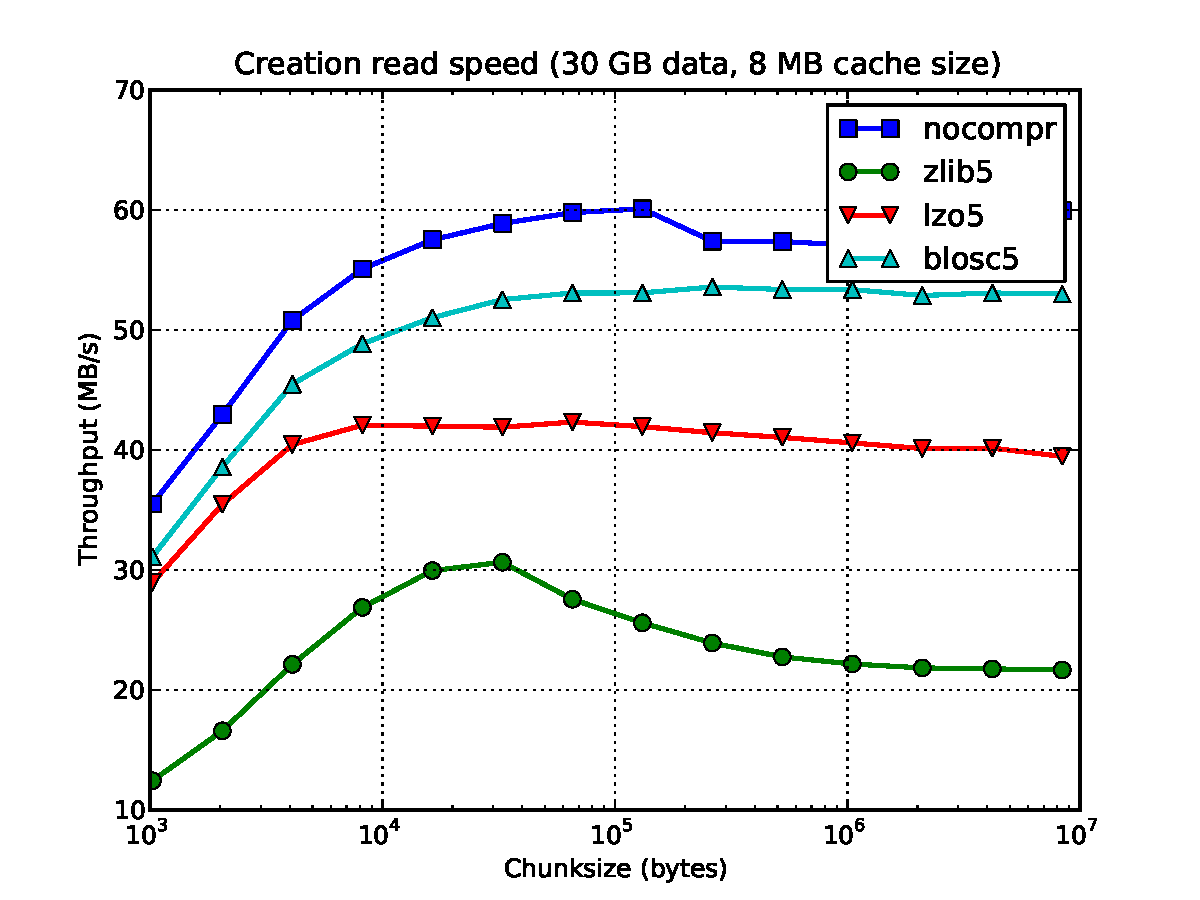
\includegraphics[scale=0.4]{create-chunksize-30GB}
\par\end{center}


\lyxframeend{}\lyxframe{Effect of chunked compression when reading large datasets}

\begin{center}
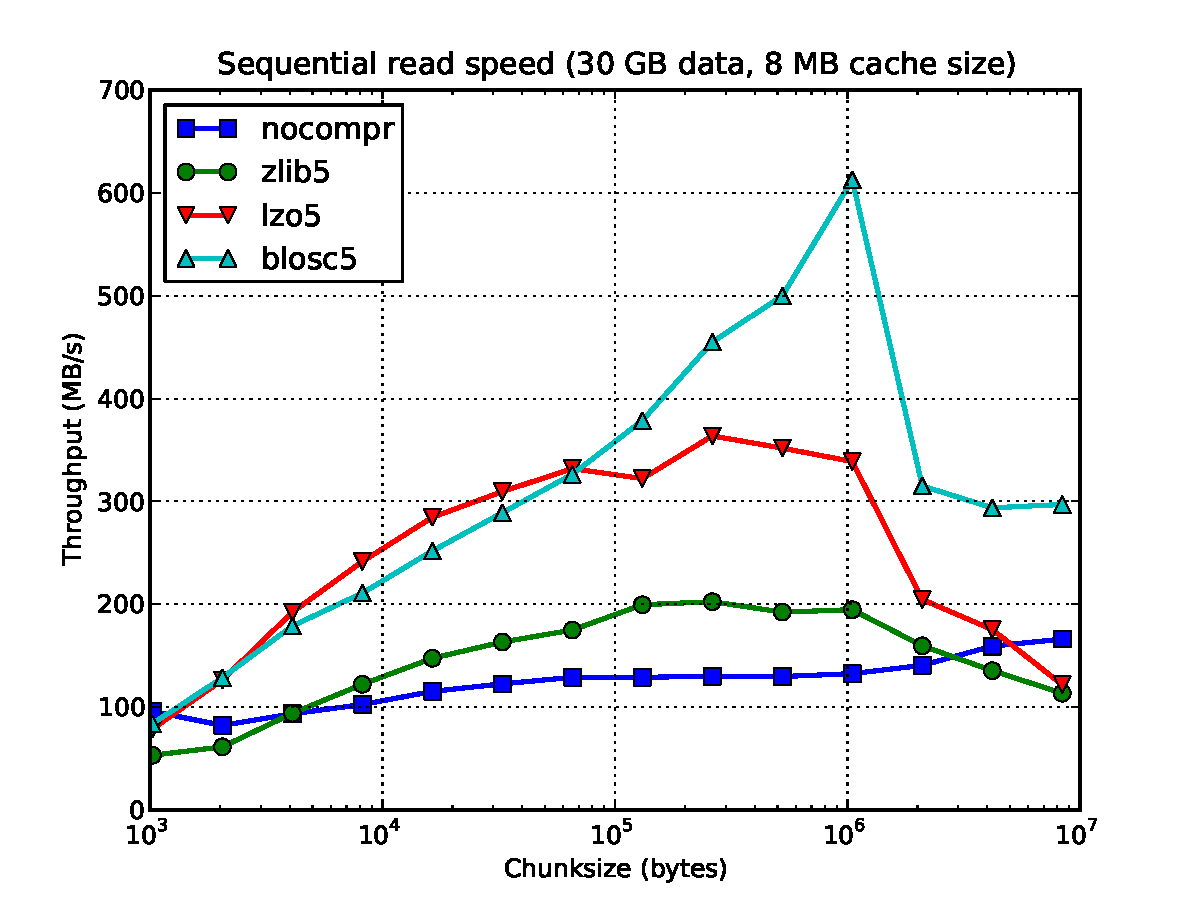
\includegraphics[scale=0.4]{sequential-8MB-30GB}
\par\end{center}


\lyxframeend{}\lyxframe{When should you use compression?}
\begin{itemize}
\item Your data has to be compressible (sparse matrices, time series, data
with low entropy, ...).
\item Whether your disk space is tight or your datasets are large.
\item You want to optimize I/O speed.
\item It's fun!
\end{itemize}

\lyxframeend{}\section*{Summary}


\lyxframeend{}\lyxframe{Summary}
\begin{itemize}
\item Pickle is the most basic, but still powerful, way to serialize Python
data. But it is mainly meant for small datasets and it is not portable.
\item Relational databases are portable, mature and solid as a rock. However,
they do not interact well with NumPy and write performance is pretty
lame.
\item HDF5 / NetCDF4 formats show best performance, Python APIs interacts
well with NumPy and are extremely portable. They lack safety features.
\item Using compression allows you to deal with more data using the same
resources. In general, they can save I/O time to disk.
\end{itemize}

\lyxframeend{}\lyxframe{More Info}

\beamertemplatebookbibitems
\begin{thebibliography}{3}
\bibitem{Beazley2009}David Beazley \newblock Python -- Essential
Reference \newblock Addisson-Wesley,2009\beamertemplatearticlebibitems

\bibitem{Kern2007}Robert Kern \newblock\emph{ NPY: A Simple File
Format for NumPy Arrays} \newblock NumPy Enhancement Proposal, December
2007\beamertemplatearrowbibitems

\bibitem{key-1}The HDF Group \newblock\emph{ }What is HDF5?\newblock
\url{http://www.hdfgroup.org/HDF5/whatishdf5.html}

\end{thebibliography}

\lyxframeend{}\lyxframe{Thank You!}

Contact:

\begin{center}
\textcolor{red}{faltet@pytables.org}
\par\end{center}


\lyxframeend{}
\end{document}
